
    \documentclass{article}

    %  Русский язык

    \usepackage[T2A]{fontenc}			% кодировка
    \usepackage[utf8]{inputenc}			% кодировка исходного текста
    \usepackage[english,russian]{babel}	% локализация и переносы
    \usepackage{unicode-math}
    \usepackage[top=3in]{geometry}

    % Рисунки
    \usepackage{graphicx, float}
    \usepackage{wrapfig}

    \usepackage{eso-pic,graphicx}   

    \usepackage{xcolor}

    \makeatletter
    \newcommand{\globalcolor}[1]{%
    \color{#1}\global\let\default@color\current@color
    }
    \makeatother

    \AtBeginDocument{\globalcolor{black}}

    \title{Wild wild west derivative counter}
    \author{Marty Bebrou Smith}
    \date{November 1897}

    \begin{document}
    \maketitle
    \AddToShipoutPictureBG{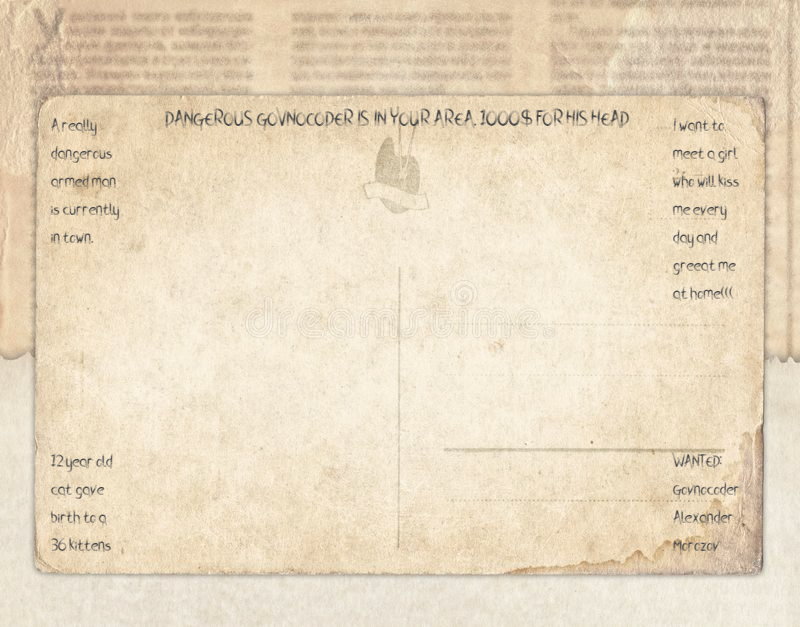
\includegraphics[width=\paperwidth,height=\paperheight]{funny_pics/back5.png}}
    

        You've been slepping so long, that Calculus anigilated all humanity and whole modern civilization was vanished.
        The humanity had to start over to restore all knowledge we lost. Unfortunately, everyone decided to become stupid cowboys and
        live in the world of Wild Wild West.

        I fucking like this live, you can bang as many hot chicks as you want, despite sometimes fuckers like you come to me
        to solve this boring equations and take derivatives.

        Oh look, a nigger is running down the hill *bang* *bang*
        
        
        Ok, ok, let's calculate this bullshit.

        \begin{center}\begin{center} 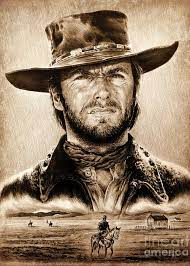
\includegraphics[scale=0.6]{funny_pics/cowboy.jpg} \end{center}\end{center}
        \begin{center}
        $\clubsuit$~$\clubsuit$~$\clubsuit$
        \end{center}

    \begin{center} 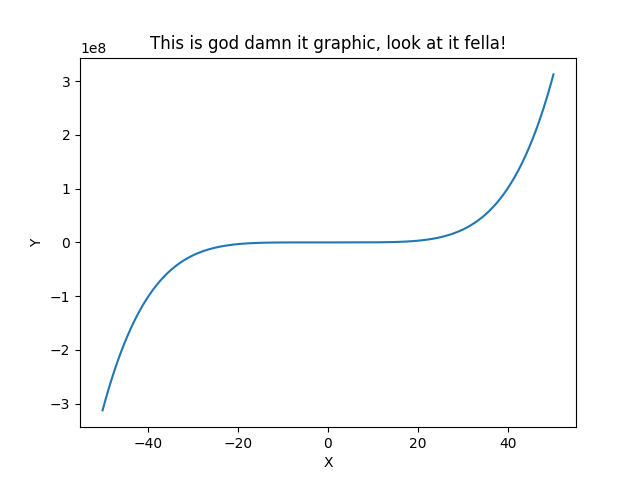
\includegraphics[scale=0.6]{function_graph.png} \end{center}Alright fella, let's look wat we got, i haven't seen so beautiful trees for ages:

\begin{center}$
{{{{({\sin{({{2}\cdot{x}})}})}^{({5})}}-{\cos{({x})}}}+{{x}^{5}}}
$\end{center}
\begin{center} $\clubsuit$~$\clubsuit$~$\clubsuit$ \end{center}\begin{center}  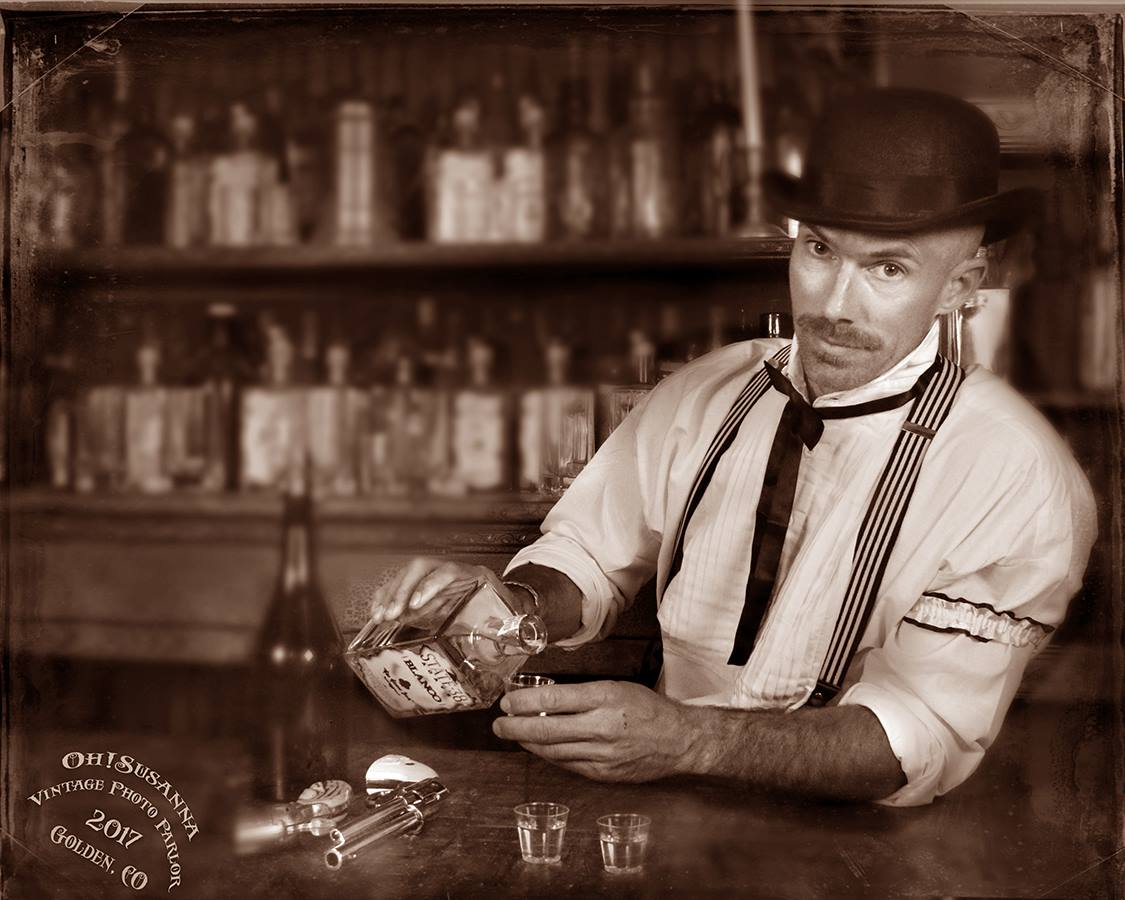
\includegraphics[scale=0.3]{funny_pics/bartender.jpg} \end{center} With the power of gods, let's write the following: 
\begin{center}$
{{({{({5})}\cdot{({{x}^{4}})}})}\cdot{({1})}}
$\end{center}
\begin{center} $\clubsuit$~$\clubsuit$~$\clubsuit$ \end{center}\begin{center}  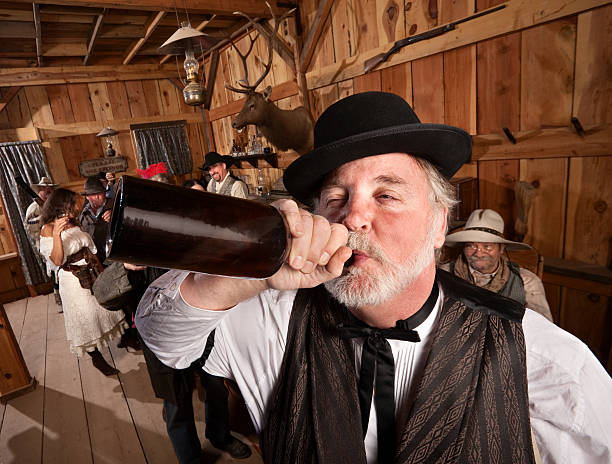
\includegraphics[scale=1.4]{funny_pics/drunk_cowboy.jpg} \end{center} I smacked a damn big cockroach yesterday fella, this was left on my shoe: 
\begin{center}$
{{({{({-1})}\cdot{({\sin{({x})}})}})}\cdot{({1})}}
$\end{center}
\begin{center} $\clubsuit$~$\clubsuit$~$\clubsuit$ \end{center}\begin{center} 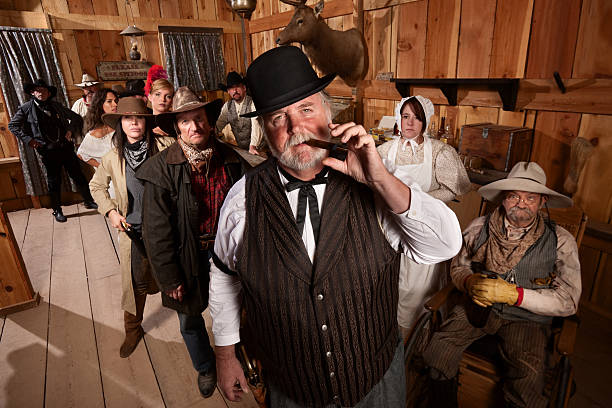
\includegraphics[scale=1.4]{funny_pics/funny_bartender.jpg} \end{center} Don't distract fella, I don't know how to count
\begin{center}$
{{{0}\cdot{x}}+{{2}\cdot{1}}}
$\end{center}
\begin{center} $\clubsuit$~$\clubsuit$~$\clubsuit$ \end{center}\begin{center}  
\includegraphics[scale=0.3]{funny_pics/cowboy_cat.jpg} \end{center}Oh come on, my wife is pregnant 12th time in a row.
\begin{center}$
{{({\cos{({{2}\cdot{x}})}})}\cdot{({2})}}
$\end{center}
\begin{center} $\clubsuit$~$\clubsuit$~$\clubsuit$ \end{center}\begin{center}  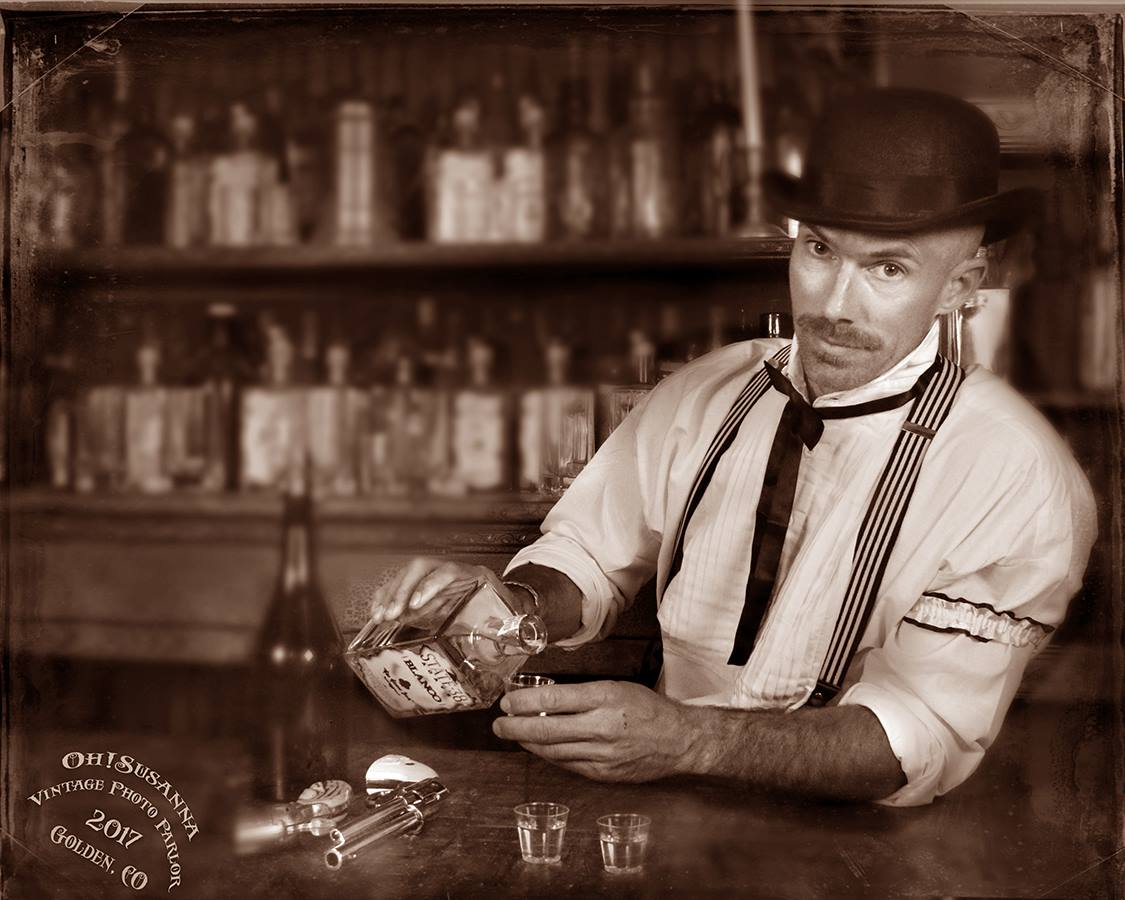
\includegraphics[scale=0.3]{funny_pics/bartender.jpg} \end{center}Can you understand it by yourself, i must go get some beer, fella:
\begin{center}$
{{({{({5})}\cdot{({{({\sin{({{2}\cdot{x}})}})}^{({4})}})}})}\cdot{({{({\cos{({{2}\cdot{x}})}})}\cdot{({2})}})}}
$\end{center}
\begin{center} $\clubsuit$~$\clubsuit$~$\clubsuit$ \end{center}...
\begin{center}$
{{{({{({5})}\cdot{({{({\sin{({{2}\cdot{x}})}})}^{({4})}})}})}\cdot{({{({\cos{({{2}\cdot{x}})}})}\cdot{({2})}})}}-{{({{({-1})}\cdot{({\sin{({x})}})}})}\cdot{({1})}}}
$\end{center}
\begin{center} $\clubsuit$~$\clubsuit$~$\clubsuit$ \end{center}\begin{center}  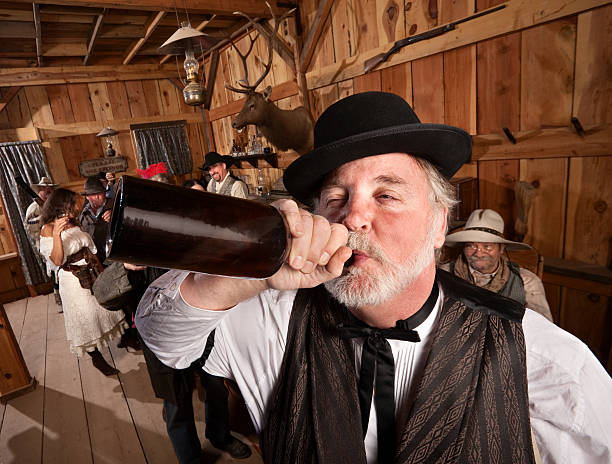
\includegraphics[scale=1.4]{funny_pics/drunk_cowboy.jpg} \end{center}Thanks man
\begin{center}$
{{{{({{({5})}\cdot{({{({\sin{({{2}\cdot{x}})}})}^{({4})}})}})}\cdot{({{({\cos{({{2}\cdot{x}})}})}\cdot{({2})}})}}-{{({{({-1})}\cdot{({\sin{({x})}})}})}\cdot{({1})}}}+{{({{({5})}\cdot{({{x}^{4}})}})}\cdot{({1})}}}
$\end{center}
\begin{center} $\clubsuit$~$\clubsuit$~$\clubsuit$ \end{center}Here is whach you got, fella. Now let's drink some whiskey and shoot niggers.\begin{center} 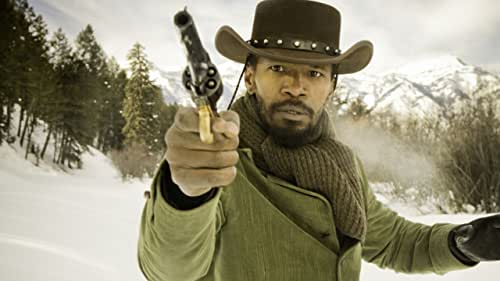
\includegraphics[scale=0.6]{funny_pics/slave.jpg} \end{center}
\begin{center}$
{{{{({{({5})}\cdot{({{({\sin{({{2}\cdot{x}})}})}^{({4})}})}})}\cdot{({{({\cos{({{2}\cdot{x}})}})}\cdot{({2})}})}}-{{({{({-1})}\cdot{({\sin{({x})}})}})}\cdot{({1})}}}+{{({{({5})}\cdot{({{x}^{4}})}})}\cdot{({1})}}}
$\end{center}
\begin{center} $\clubsuit$~$\clubsuit$~$\clubsuit$ \end{center}Alright fella, let's make this shit called Macloren,there will be only 3 steps, cause i don't know how to count more.Basicly the main formula will look like that
 \[ f(x) = f(0) + \frac{f^{(1)}(0)}{1!}\cdot X + \frac{f^{(2)}(0)}{2!}\cdot X + \frac{f^{(3)}(0)}{3!}\cdot X + \text{...}\]
\[ f^{(0)}(0) = -1\]\[ f^{(1)}(0) = 0\]\[ f^{(2)}(0) = 1\]\[ f^{(3)}(0) = 0\]
        The solution is pretty simple and you definetely can do it \textbf{yourself}
        \end{document}
    